\section{Figures}

\begin{figure}[H]
\centering
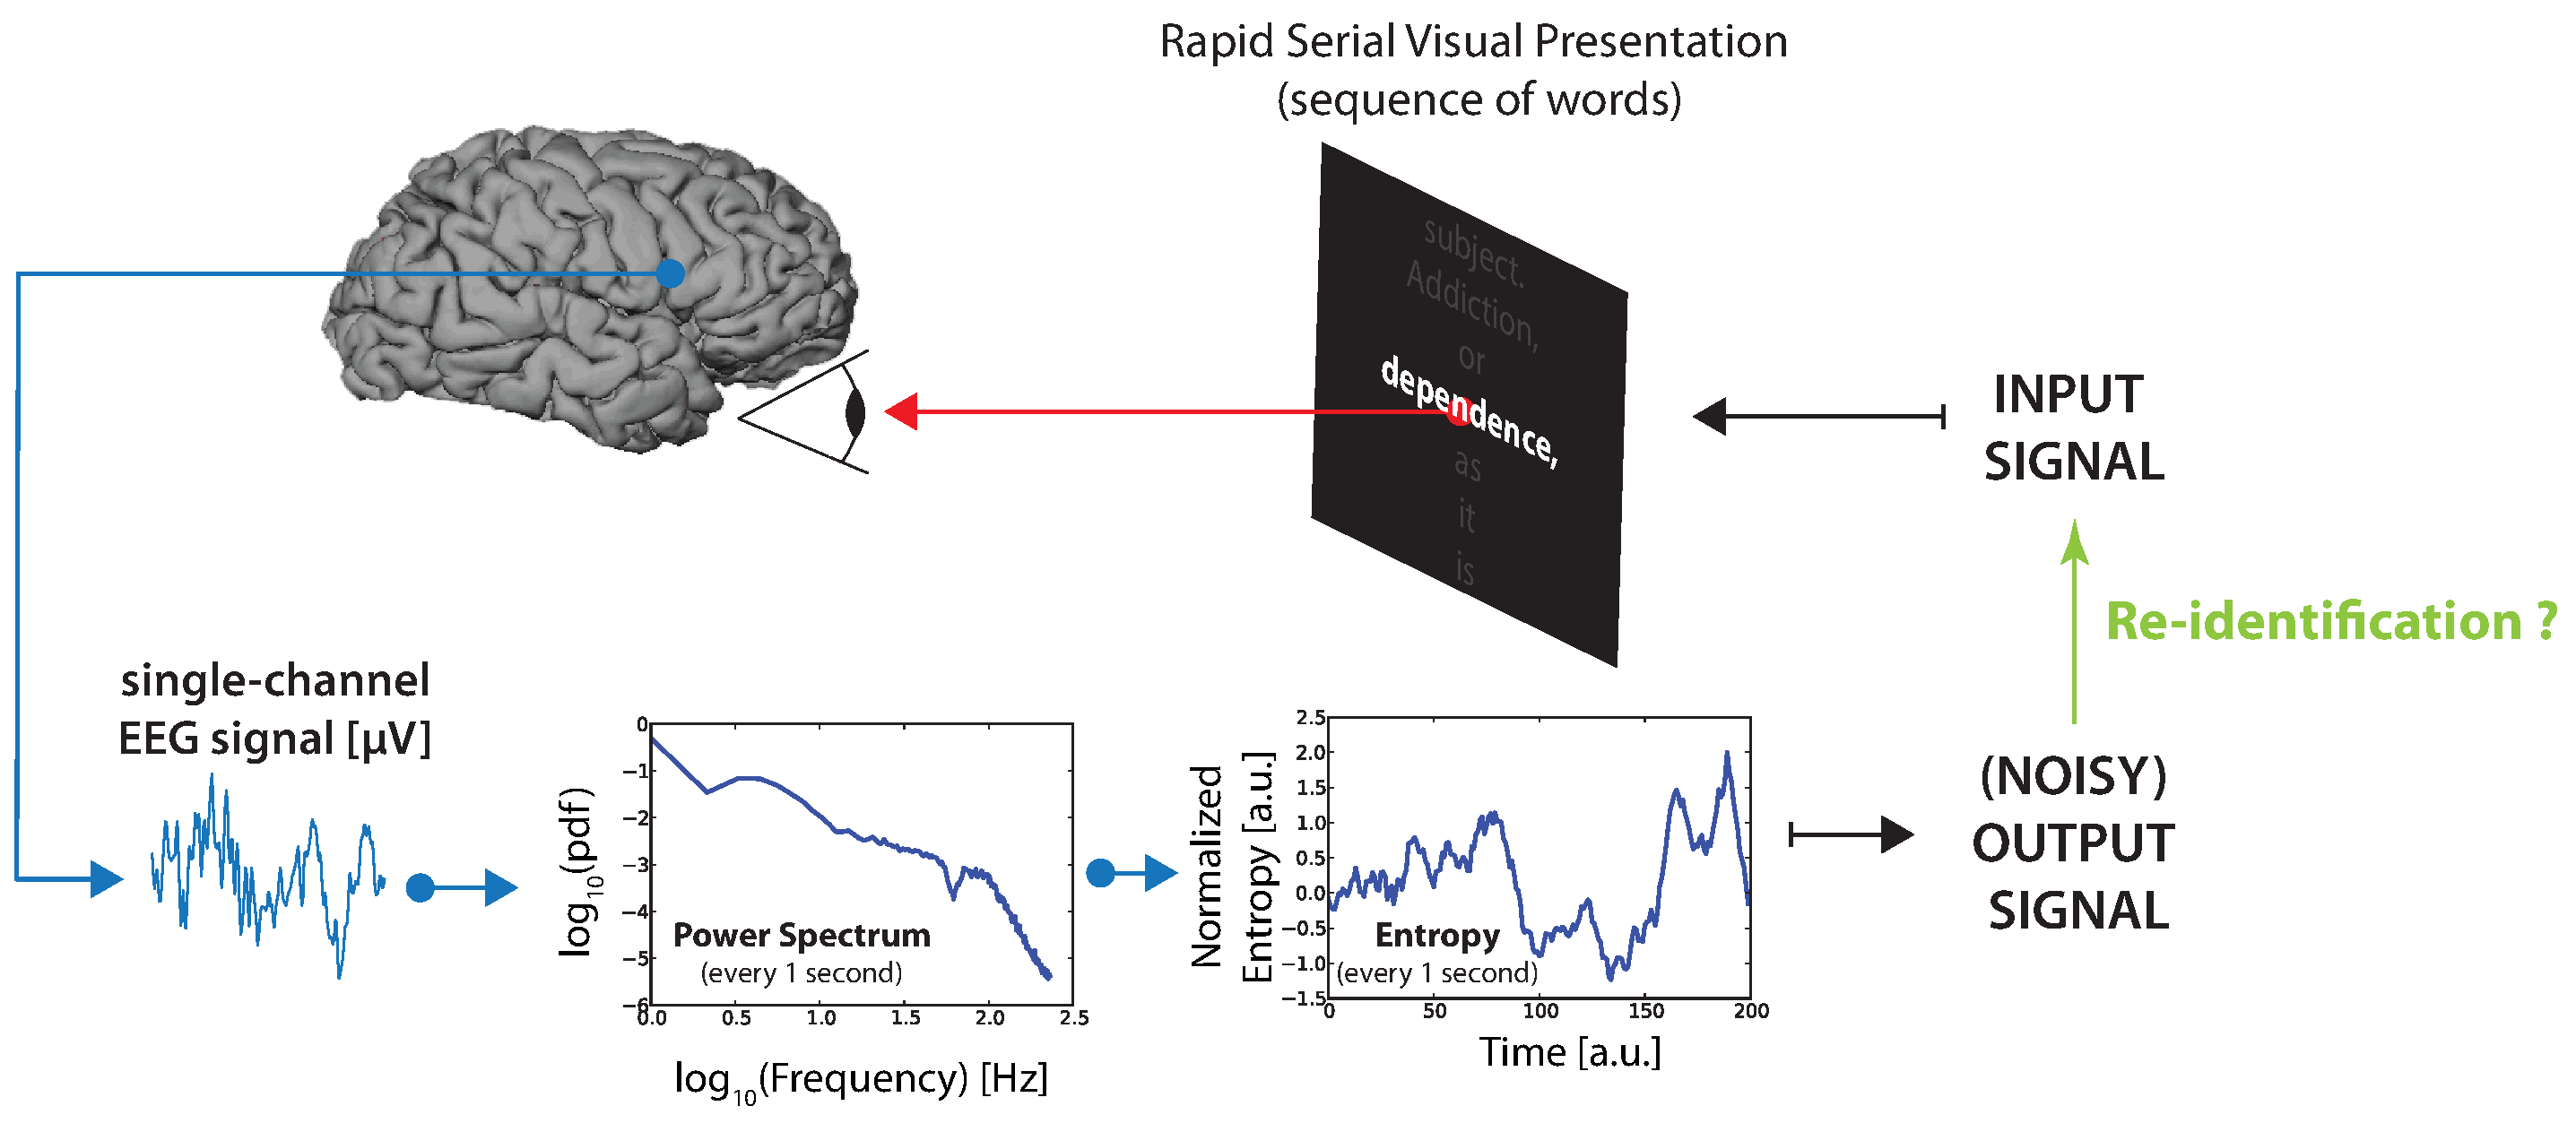
\includegraphics[width=17cm]{figures/main.eps}
\caption{Experimental setting: A text is displayed as a sequence of words on a black screen at a rate of 125 milliseconds per word. The EEG signal is captured by a rudimentary EEG dry electrode positioned on the left forehead ({\bf Fp9} in the 10-20 electrodes position system). Each time a word is displayed the power spectrum of the signal is computed over the last second of EEG signal. The information contained on the power spectrum is then {\it compressed} as a measure of entropy (see formula \ref{entropy}). The entropy is most commonly associated with a measure of disorder of signal. Here, measuring the entropy of the power spectrum of the EEG signal is equivalent to a rough metric of the level of disorder of EEG wave modulations occurring in the brain over a short period.}
\label{fig:apparatus}
\end{figure}

\clearpage

\begin{figure}[H]
\centering
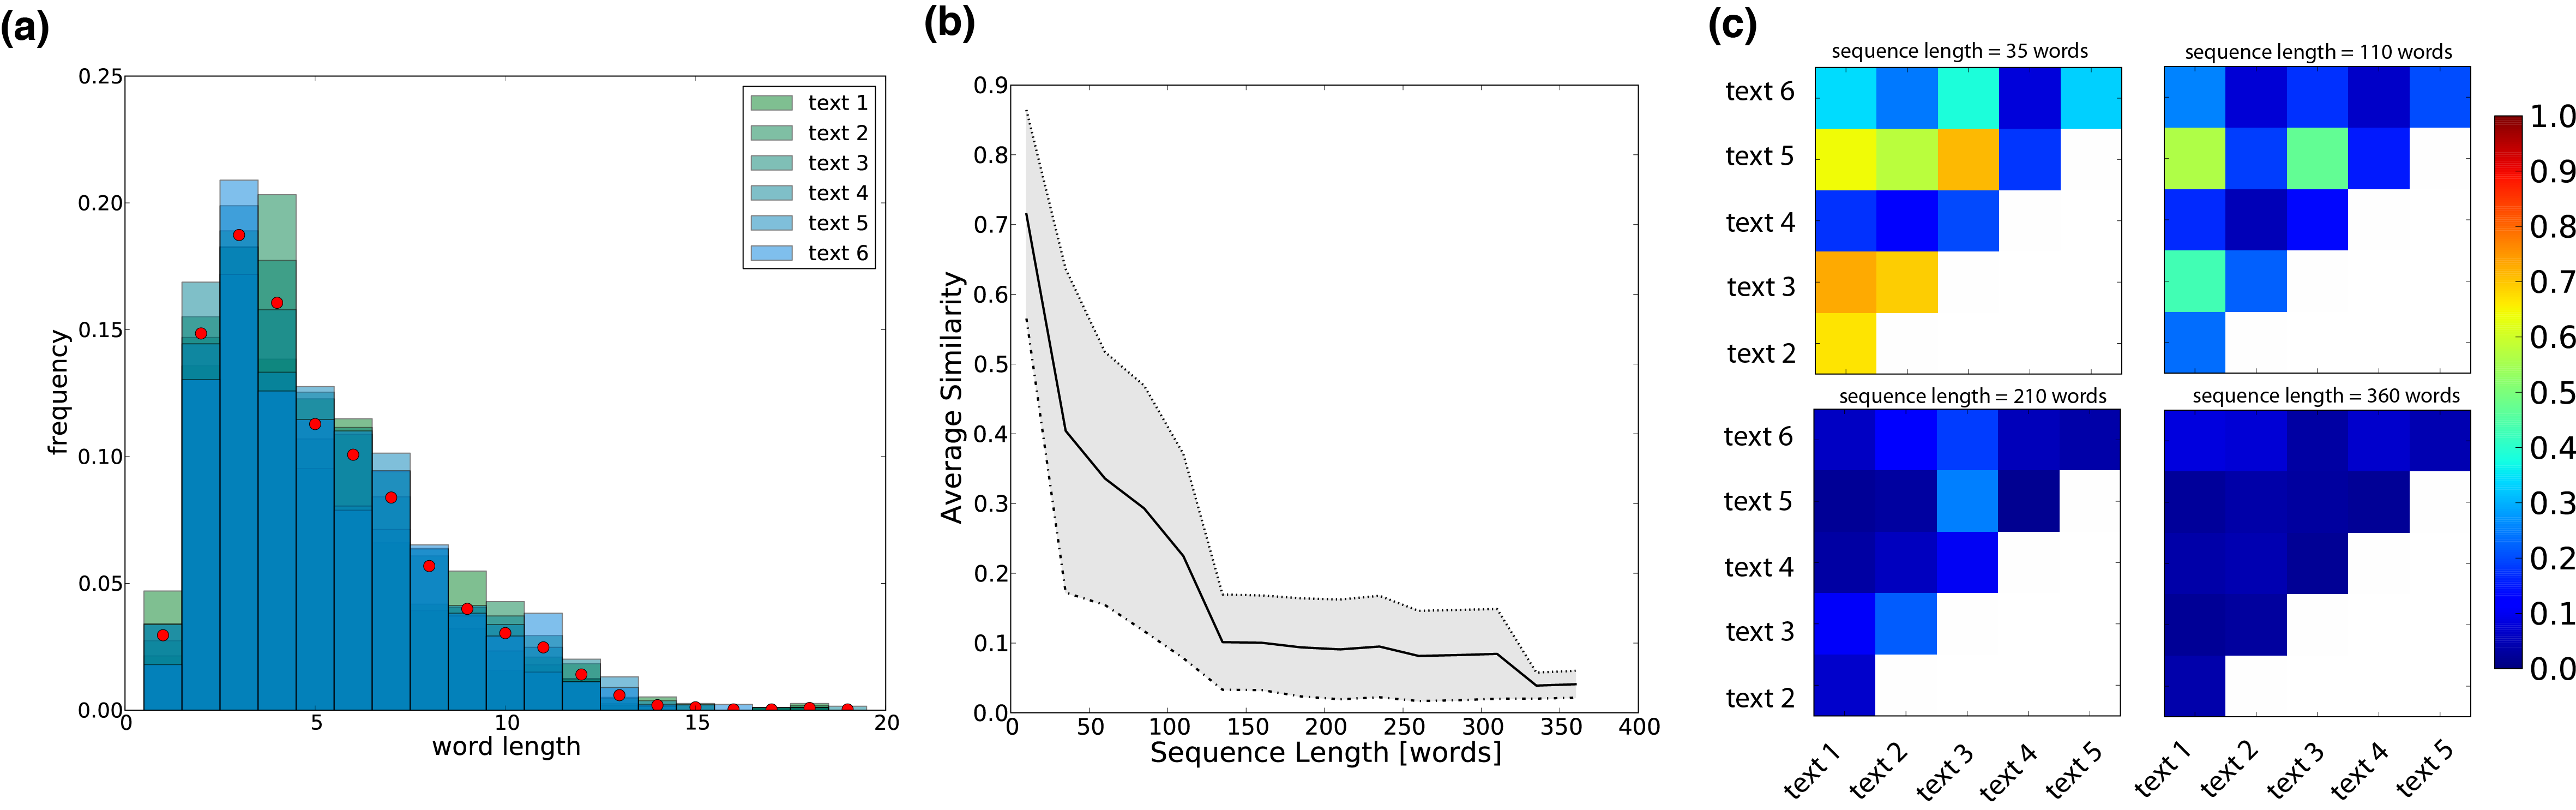
\includegraphics[width=17cm]{figures/word_density.png}
\caption{{\bf a.} One must define what may cause disorder in the brain: Here, we assume that disorder is caused by less expected or less common words, which require a higher level of cognitive processing. The probability distribution of word occurrence in a text is unique, and the arrangement of these words is even more unique (see Figure \ref{fig:sequences} below). Nevertheless, the distribution of probabilities of words is in general quite stable across texts. As shown here, the density function of word follows roughly the same pattern: words with approx. 5 characters are most common; one-character words are less frequent, and the larger words the more their frequency diminishes. Over large corpus of words, it has been found that the frequency of words with size $s$ or larger follows a power law given as $\sim 1/s$ \cite{wordfreq}. In other words, a word made of 10 characters has a chance to appear every ten words. Here, the distribution of a rather small piece of text is also skewed, but typically not as heavy-tailed as a whole corpus because there are not enough words in the text to have the tail distribution explored (e.g. words  with more than 20 or 30 characters) by the law of large numbers. {\bf b.} Similarity between texts (table/matrix with cossim measures?).}
\label{fig:wl_distribution}
\end{figure}


\clearpage


\begin{figure}[H]
\centering
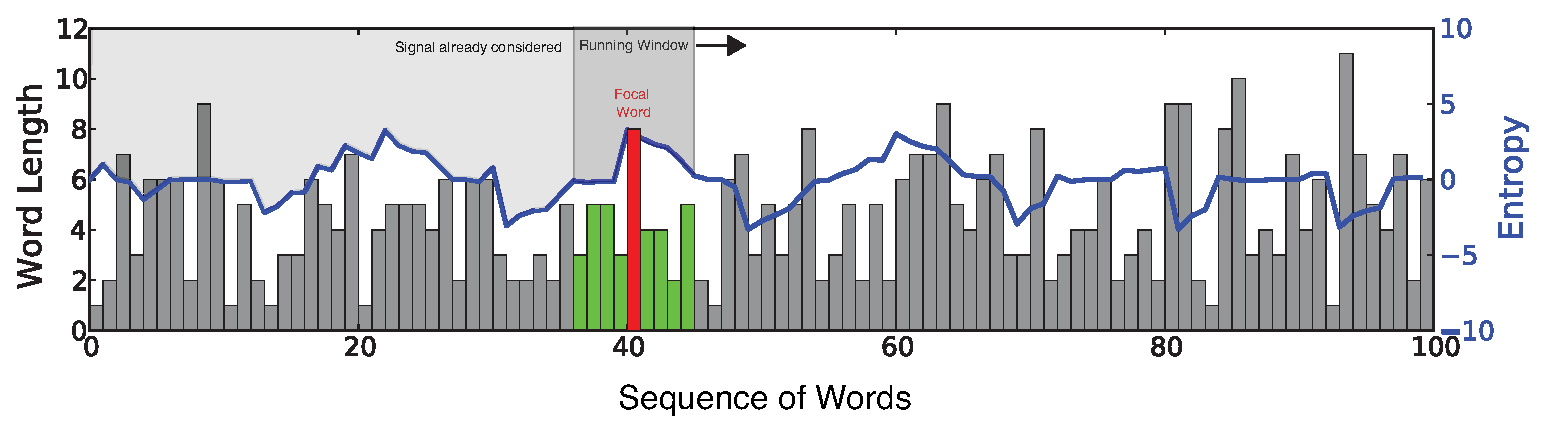
\includegraphics[width=15cm]{figures/lWordsEntropyTimeline.eps}
\caption{Typical sequence of entropy (blue) associated with each word. The entropy signal is smoothed by taking the sum of entropies in the vicinity of the focal word. The entropy shall be considered as the noisy signal as a result of the {\it processing} of the word sequence by the brain, and captured by the dry electrode positioned on {\bf Fp9}. Re-identification of the text read requires to establish a significant correspondence between the nature of words (here their length in grey) and the entropy. The sequence length required to re-identify the text read is unknown, and thus the re-identification method starts with the first word and the first entropy measure, and continues until sufficient confidence is reached. Note that each time a new pair of word length and entropy is considered, some information as well as noise are added simultaneously. Thus, it is not certain that considering a longer sequence will add more useful information.}
\label{fig:sequences}
\end{figure}

%\caption{{\bf a.} Schematic representation of the balance of rate change $\Delta_{rate}$ as a function of word length $l_{words}$. The color gradient shows schematically the word density conditioned on their length. This is the canonical or most desirable situation: Around the mean word length the deterministic component of $\Delta_{rate}$ is close to zero. For words with length smaller, the deterministic part of the rate increases, while for words with length larger than the mean, the rate is decreased. The dotted line shows another possible configuration, with acceleration occurring when words are longer. Empirical evidence for the latter case is shown  in Figure \ref{fig:examples} for some typical successful and failed attempts to maintain a balance. ({\bf c}) The joint probability density function $pdf( \Delta_{rate} \times l_{words})$ is well balanced, yet skewed, showing that good control is achieved, along with a good capacity to change the rate of word display.}
%
%%The linear regression of the average $\Delta_{rates}$ for each word length (for $l_{words} < 10$) exhibits a slope $= 4(1)\times10^{-3}$ ($p < 0.01$). The intersection of $l_{words}(\Delta_{rates} =0) = 4.43$ very close to the average word length (in the text). The error bars show the dispersion (standard deviation of  $\Delta_{rates}$ for each word length. This dispersion is rather large reflecting the stochastic nature of complex brain activation sand the coarse measure obtained from the single electrode EEG headset.
%
%\begin{figure}[H]
%\centering
%\includegraphics[width=12cm]{../figures2/examples.eps}
%\caption{Four examples of successful and failed neuro-feedback control strategies. For each case, three panels are shown (from left to right): (i) Evolution of rate at each displayed word, (ii) rate change as a function of word length at each time step, and (iii)  rate change in the vicinity of large words (9 or more characters, red line), versus words with smaller than 5 characters (blue). The 90\% confidence intervals (light blue area) are obtained by replacement bootstrapping (100 samples of same size as large words are randomly drawn from small words). {\bf a.} Illustration of a very well controlled RSVP, with a sharp and localized drop of word presentation rate around the time large word occurrence. {\bf b.} Opposite strategy with rate increased around large words. {\bf c.} Yet another neuro-feedback strategy with the rate being controlled after the word has occurred. {\bf d.} Failed strategy: Compared to {\bf a}, {\bf b} and {\bf c} the rate change is consistently negative, hence dragging RSVP towards the lower rate limit. Note also in {\bf c} how the rate change as a function of word length (middle panel) is unbalanced around the 0-rate change (horizontal black line) and the mean word length (vertical black line), on the  contrary to {\bf a}, {\bf b} and {\bf c}.}
%\label{fig:examples}
%\end{figure}
%
%
%\begin{figure}[H]
%\centering
%%\includegraphics[width=12cm]{../figures2/examples.eps}
%\caption{Here a figure on how the rate is influenced by the power septrum. The idea is to cherry pick moments of high rate change, and look how the power spectrum (and entropy) influences these changes (keep in mind the smoothing, which should reduce the effects of pSpectrum changes on the rate.).}
%\label{fig:S_vs_rate}
%\end{figure}
%
%\begin{figure}[H]
%\centering
%%\includegraphics[width=12cm]{../figures2/examples.eps}
%\caption{To measure whether there is an effect in the constant rate case, one must first reverse engineer how the rate influences some power spectrum, and how it influences the rate}
%\label{fig:constant_rate}
%\end{figure}



